\chapter{Analysis Of The Problem}\label{sec:chap:3}

The number of mobile users is increasing dramatically, translating into an increasing demand of mobile data services. Mobile data traffic increased by 81\% in 2013 and by 69\% in 2014 \cite{internet_trends} and the rate of increase is not slowing down. 5G, the mmWave, is disruptive upcoming technology that employs frequencies in the order of 60GHz that will impose very high requirements, given the extremely high bandwidths it will provide in very small areas \cite{5g}. This has a direct correlation with both the increased accesibility to the internet from mobile devices via WLANs and RANs, and the increase in popularity of applications designed for smartphones and tablets. On top of this, operators are migrating their networks to full IP based networks for both voice and data \cite{fama}.

\begin{center}
\begin{figure}[h!]
  \centering
    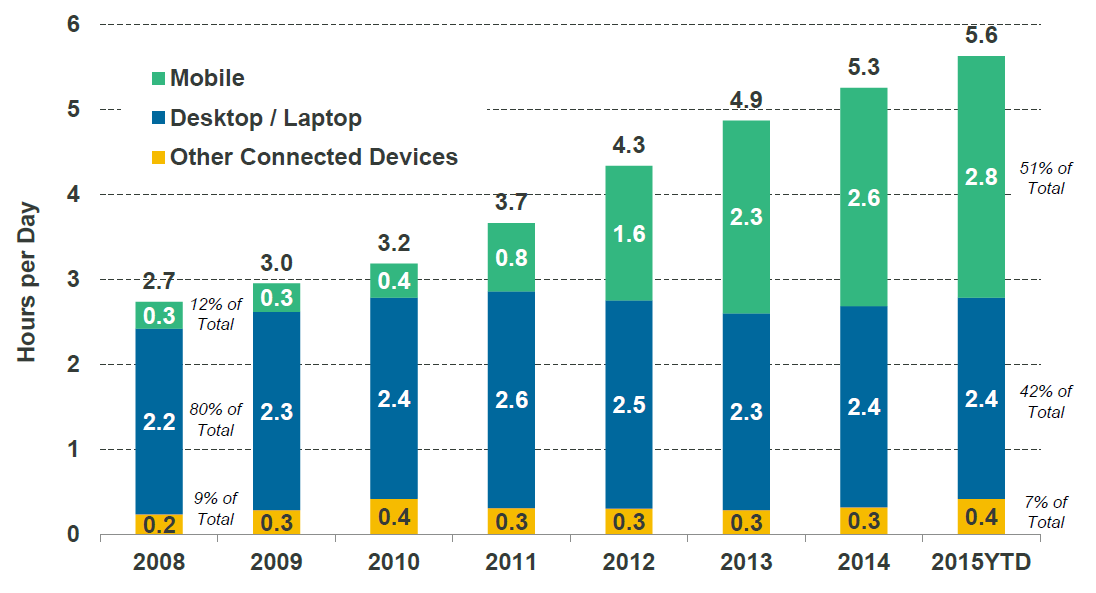
\includegraphics[scale=0.4]{./images/traffic_data}
	\caption{Mobile Traffic Data}
	\label{traffic_data-fig}
\end{figure}
\end{center}

Current centralized mobility management solutions include protocols such as Mobile IPv6 or Proxy Mobile IPv6. These protocols depend on a centralized entity for mobility management and data forwarding. This makes these solutions vulnerable to problems such as:

\begin{itemize}
\item{\textbf{Sub-optimal routing}}
\item{\textbf{Scalability}}
\item{\textbf{Signaling overhead}}
\item{\textbf{Complex network deployment}}
\item{\textbf{Lake of granular network control}}
\item{\textbf{Single point of failure}}
\end{itemize}

On the other hand, interference due to uncoordinated resource sharing techniques reprensents a key limiting factor in the design of dense wireless networks \cite{sdn_dense}.\\

The solution proposed in this project is a combination of Software Defined Networking and Distribted Mobility Management to tackle these problems.









